%-------------------------------------------------------------------------------
%                      Template Naskah Skripsi
%               	Berdasarkan format Teknik Mesin UII 
% 						(c) @Edi SN 2020
%-------------------------------------------------------------------------------

%Template pembuatan naskah skripsi.
\documentclass{TMUIITA}

%Untuk prefiks pada daftar gambar dan tabel
\usepackage[titles]{tocloft}
\renewcommand\cftfigpresnum{Gambar\  }
\renewcommand\cfttabpresnum{Tabel\   }

%Untuk hyperlink dan table of content
\usepackage{hyperref}
\newlength{\mylenf}
\settowidth{\mylenf}{\cftfigpresnum}
\setlength{\cftfignumwidth}{\dimexpr\mylenf+2em}
\setlength{\cfttabnumwidth}{\dimexpr\mylenf+2em}

%Untuk Bold Face pada Keterangan Gambar
\usepackage[labelfont=bf]{caption}

%Untuk caption dan subcaption
\usepackage{caption}
\usepackage{subcaption}


%-----------------------------------------------------------------
%Disini awal masukan untuk data proposal skripsi
%-----------------------------------------------------------------
\titleind{karakterisasi aspek afektif pada permukaan
menggunakan fitur berbasis fourier transform}

\fullname{Edi Setyawan Nugroho}

\idnum{16525070}

\NIRM {2016070535}

\approvaldate{3 Februari 2014}

\degree{Sarjana Teknik Mesin}

\yearsubmit{2020}

\program{Teknik Mesin}

\dept{Teknik Mesin}

\firstsupervisor{Mohammad Faizun, S.T., M.Eng., Ph.D.}
\firstnip{NIP}

%\secondsupervisor{Bimo Sunarfri Hantono, S.T., M.Eng.}
%\secondnip{1977 0131 2002 12 1 003}

%-----------------------------------------------------------------
%Disini akhir masukan untuk data proposal skripsi
%-----------------------------------------------------------------

\begin{document}

\cover

\approvalpage

\pengesahanpage


%-----------------------------------------------------------------
%Disini awal masukan Acknowledment
%-----------------------------------------------------------------
\acknowledgment
\begin{flushright}
\emph{Untuk Ibu, Bapak,\\dan Adikku tercinta.}
\end{flushright}
%------------------------------------------------
%Disini massukkan motto
%------------------------------------------------
\mottopage
%-----------------------------------------------------------------
%Disini awal masukan untuk Prakata
%-----------------------------------------------------------------
\preface
Assalamu'alaikum Wr. Wb.

\vspace{0.5cm}

Puji syukur penulis panjatkan ke hadirat Allah SWT karena hanya dengan rahmat dan hidayah-Nya, Tugas Akhir ini dapat terselesaikan tanpa halangan berarti. Keberhasilan dalam menyusun laporan Tugas Akhir ini tidak lepas dari bantuan berbagai pihak yang mana dengan tulus dan ikhlas memberikan masukan guna sempurnanya Tugas Akhir ini. Oleh karena itu dalam kesempatan ini, dengan kerendahan hati penulis mengucapkan terima kasih kepada:

\begin{enumerate}
\item{Bapak Risdiyono, S.T., M.Eng., Ph.D., selaku Ketua Jurusan Teknik Mesin  Fakultas Teknologi Industri Universitas Islam Indonesia,}
\item{Bapak Mohammad Faizun, S.T., M.Eng., Ph.D selaku dosen pembimbing yang telah memberikan banyak bantuan, bimbingan, serta arahan dalam Tugas Akhir ini,}

\item{Bapak Dr. Ir. Paryana Puspaputra, M.Eng. selaku dosen pembimbing akademis penulis,}
\item{Seluruh Dosen di Jurusan Teknik Mesin Fakultas Teknologi Industri Universitas Islam Indonesia, yang tidak bisa disebutkan satu-satu, atas ilmu dan bimbingannya selama penulis berkuliah di Jurusan Teknik Mesin FTI UII,}
\item{Ibu dan Bapak yang selama ini telah sabar membimbing, mengarahkan, dan mendoakan penulis tanpa kenal lelah untuk selama-lamanya.}

\end{enumerate}

Penulis menyadari bahwa penyusunan Tugas Akhir ini jauh dari sempurna. Kritik dan saran dapat ditujukan langsung pada e-mail saya. Akhir kata penulis mohon maaf yang sebesar-besarnya apabila ada kekeliruan di dalam penulisan Tugas Akhir ini.

\vspace{0.5cm}

Wassalamu'alaikum Wr. Wb.

\begin{tabular}{p{7.5cm}c}
&Yogyakarta, 15 Januari 2014\\
&\\
&\\
&\textbf{Penulis}
\end{tabular}

%-----------------------------------------------------------------
%Disini akhir masukan untuk muka skripsi
%-----------------------------------------------------------------
\tableofcontents
\addcontentsline{toc}{chapter}{DAFTAR ISI}
\listoftables
\addcontentsline{toc}{chapter}{DAFTAR TABEL}
\listoffigures
\addcontentsline{toc}{chapter}{DAFTAR GAMBAR}

%-----------------------------------------------------------------
%Daftar Singkatan [Optional]
%-----------------------------------------------------------------
\singkatan
\noindent

\begin{tabular}{p{20pt}p{3pt}l}
\textbf{A}\\
AJAX & & Asynchronous JavaScript and XML\\
AP & & Access Point\\
API & & Application Programming Interface\\
\\
\end{tabular}

\begin{tabular}{p{20pt}p{3pt}l}
\textbf{C}\\
CLI & & Command Line Interface\\
\\
\end{tabular}

\begin{tabular}{p{20pt}p{3pt}l}
\textbf{C}\\
DFM & & Discovered Full Mesh\\
\\
\end{tabular}

\begin{tabular}{p{20pt}p{3pt}l}
\textbf{E}\\
ERD & & Entity Relationship Diagram\\
\\
\end{tabular}

\begin{tabular}{p{20pt}p{3pt}l}
\textbf{F}\\
FTDI & & Future Technology Devices International\\
FUSE & & Filesystem in Userspace\\
\\
\end{tabular}

\begin{tabular}{p{20pt}p{3pt}l}
\textbf{I}\\
IP & & Internet Protocol\\
\\
\end{tabular}

\begin{tabular}{p{20pt}p{3pt}l}
\textbf{J}\\
JTETI & & Jurusan Teknik Elektro dan Teknologi Informasi\\
\\
\end{tabular}

\begin{tabular}{p{20pt}p{3pt}l}
\textbf{L}\\
LAN & & Local Area Network\\
\\
\end{tabular}

\begin{tabular}{p{20pt}p{3pt}l}
\textbf{O}\\
OSI & & Open Systems Interconnection\\
\\
\end{tabular}

\begin{tabular}{p{20pt}p{3pt}l}
\textbf{R}\\
RF & & Radio Frequency\\
\\
\end{tabular}

\begin{tabular}{p{20pt}p{3pt}l}
\textbf{S}\\
SDLC & & Software Development Life Cycle\\
SFTP & & Secure Shell File Transfer Protocol\\
SSHFS & & Secure Shell Filesystem\\
\\
\end{tabular}

\begin{tabular}{p{20pt}p{3pt}l}
\textbf{U}\\
UGM & & Universitas Gadjah Mada\\
USB & & Universal Serial Bus\\
\\
\end{tabular}

\begin{tabular}{p{20pt}p{3pt}l}
\textbf{V}\\
VRS & & Virtual Routing Structure\\
\\
\end{tabular}

\begin{tabular}{p{20pt}p{3pt}l}
\textbf{W}\\
WAP & & Wireless Access Point\\
WIT & & Western Indonesian Time\\
WLAN & & Wireless Local Area Network\\
WSN & & Wireless Sensor Network\\
\end{tabular}

%-----------------------------------------------------------------
%Disini awal masukan Intisari
%-----------------------------------------------------------------
\begin{abstractind}
Lorem ipsum dolor sit amet, consectetur adipisicing elit, sed do eiusmod tempor incididunt ut labore et dolore magna aliqua. Ut enim ad minim veniam, quis nostrud exercitation ullamco laboris nisi ut aliquip ex ea commodo consequat. Duis aute irure dolor in reprehenderit in voluptate velit esse cillum dolore eu fugiat nulla pariatur. Excepteur sint occaecat cupidatat non proident, sunt in culpa qui officia deserunt mollit anim id est laborum.

Sed ut perspiciatis unde omnis iste natus error sit voluptatem accusantium doloremque laudantium, totam rem aperiam, eaque ipsa quae ab illo inventore veritatis et quasi architecto beatae vitae dicta sunt explicabo. Nemo enim ipsam voluptatem quia voluptas sit aspernatur aut odit aut fugit, sed quia consequuntur magni dolores eos qui ratione voluptatem sequi nesciunt.


\bigskip
\noindent
\textbf{Kata kunci :} \emph{wireless sensor network}, \emph{Internet Protocol}, WiFi, interoperabilitas.
\end{abstractind}

\begin{abstracteng}
\emph{
Lorem ipsum dolor sit amet, consectetur adipisicing elit, sed do eiusmod tempor incididunt ut labore et dolore magna aliqua. Ut enim ad minim veniam, quis nostrud exercitation ullamco laboris nisi ut aliquip ex ea commodo consequat. Duis aute irure dolor in reprehenderit in voluptate velit esse cillum dolore eu fugiat nulla pariatur. Excepteur sint occaecat cupidatat non proident, sunt in culpa qui officia deserunt mollit anim id est laborum.}

\emph{Sed ut perspiciatis unde omnis iste natus error sit voluptatem accusantium doloremque laudantium, totam rem aperiam, eaque ipsa quae ab illo inventore veritatis et quasi architecto beatae vitae dicta sunt explicabo. Nemo enim ipsam voluptatem quia voluptas sit aspernatur aut odit aut fugit, sed quia consequuntur magni dolores eos qui ratione voluptatem sequi nesciunt.}

\bigskip
\noindent
\textbf{\emph{Keywords :}} \emph{wireless sensor network, Internet Protokol, WiFi, interoperability}.
\end{abstracteng}
%-----------------------------------------------------------------
%Disini akhir masukan Intisari
%-----------------------------------------------------------------

%-----------------------------------------------------------------
%Disini awal masukan untuk Bab
%-----------------------------------------------------------------
%!TEX root = ./template-skripsi.tex
%-------------------------------------------------------------------------------
% 								BAB I
% 							LATAR BELAKANG
%-------------------------------------------------------------------------------

\chapter{LATAR BELAKANG}

\section{Latar Belakang Masalah}
Dewasa ini banyak produsen dari suatu produk yang mulai menjadikan hal-hal non-teknis seperti estetika, afeksi dan kenyamanan sebagai salah satu pertimbangan utama dari produk yang mereka buat. Hal ini dikarenakan pihak produsen sendiri ingin membuat suatu produk yang dapat menimbulkan ikatan emosional dengan penggunannya. Salah satu aspek agar ikatan emosional antara produk dengan pengguna adalah dengan sentuhan.\\
\indent Tekstur dari suatu permukaan produk mempunyai peran yang penting dalam terciptanya kesan emosional dari suatu produk melalui sentuhan. Ini dikarenakan tekstur merupakan suatu fitur penting yang digunakan manusia untuk memperoleh informasi melalui sentuhan. Pihak produsen atau pengembang berusaha untuk membuat produk mereka memiliki tekstur yang dapat menimbulkan kesan emosional pada pengguna seperti yang mereka inginkan. \\
\indent Saat ini perancangan dan riset dari tekstur permukaan yang dapat menimbulkan kesan emosional tertentu pada manusia menggunakan metode trial and error. Hal ini tentunya sangat merugikan produsen mengingat memakan banyak waktu dan biaya. Ini memicu banyak penelitian terkait pendekatan saintifik untuk menentukan tekstur suatu permukaan yang dapat menimbulkan kesan emosional tertentu pada manusia. Salah satu alternatif yang ditawarkan oleh penulis adalah dengan mengidentifikasi karakteristik aspek afektif dari permukaan menggunakan fitur berbasis fourier transform. 

\section{Rumusan Masalah}
\indent Berdasarkan latar belakang yang telah dipaparkan di atas maka diperoleh rumusan masalah sebagai berikut:
\begin{enumerate}
	\item Bagaimana aspek afektif dari suatu permukaan direprsentasikan dengan fitur berbasis Fourier Transform?
	\item Bagaimana aspek afektif dari suatu permukaan?
\end{enumerate}


\section{Batasan Masalah}
\indent Berdasarkan rumusan masalah tersebut pada penelitian ini akan dilakukan pembatasan masalah sebagai berikut:
\begin{enumerate}
\item Penelitian ini menggunakan subjek uji yaitu WNI dengan rentang usia dari 20 tahun sampai dengan 25 tahun.
\item Jumlah fitur yang digunakan untuk menganalisis karakter adalah 109 fitur.
\item Penyusunan terminologi yang berkaitan dengan aspek afektif berasal dari perbandingan hasil pengujian awal dengan referensi yang sudah ada.
\item Terminologi afeksi yang dipakai adalah yang tercantum dari kamus besar bahasa indonesia(KBBI).
\item Penelitian ini hanya mempelajari aspek afeksi dari sentuhan manusia pada sebuah permukaan saja.
\item Penelitian ini dibatasi hanya sampai dengan pembuatan model dan analisis hubungan antara fitur berbasis Fourier Transform dengan afeksi yang dihasilkan dari sentuhan saja.

\end{enumerate}


\section{Tujuan Penelitian}
\indent Berdasarkan rumusan masalah di atas, maka penelitian ini dilakukan dengan tujuan sebagai berikut:
\begin{enumerate}
	\item Mengetahui karakteristik aspek afektif dari suatu permukaan menggunakan fitur berbasis Fourier Transform.
	\item Mengetahui macam-macam aspek afektif yang ada pada suatu permukaan.
	\item Mengetahui hubungan antara fitur berbasis Fourier Transform dengan aspek afektif dari suatu permukaan.
\end{enumerate}


\section{Manfaat Penelitian}
\indent Terdapat beberapa manfaat dari penelitian ini untuk beberapa pihak seperti peneliti,kampus dan industri.

\subsection{Manfaat untuk Peneliti}
\begin{enumerate}[a.]
	\item Mengetahui aspek afektif dari suatu permukaan dengan metode yang lebih akurat.
	\item Mengetahui hubungan antara aspek afektif dari sentuhan dengan fitur berbasis Fourier Transform.
	\item Mengetahui karakteristik permukaan yang disukai dan tidak disukai oleh seseorang dengan fitur berbasis Fourier Transform.
\end{enumerate}

\subsection{Manfaat untuk Kampus}
\begin{enumerate}[a.]
	\item Memperoleh perspektif baru mengenai \emph{affective engineering design.}
	\item Mengetahui potensi research area disiplin ilmu teknik mesin yang berkaitan dengan disiplin ilmu lain.
\end{enumerate}

\subsection{Manfaat untuk Industri}
\begin{enumerate}[a.]
	\item Mengetahui karakteristik permukaan yang berpotensi untuk disukai/digemari konsumen.
	\item Memiliki acuan yang untuk merekayasa suatu permukaan agar produk dapat menimbulkan ikatan emosional kepada konsumen.
\end{enumerate}

\section{Sistematika Penulisan}
\noindent
\textbf{BAB I : PENDAHULUAN}

Pada bab ini dijelaskan latar belakang, rumusan masalah, batasan, tujuan, manfaat, keaslian penelitian, dan sistematika penulisan.\\

\noindent
\textbf{BAB II : TINJAUAN PUSTAKA DAN LANDASAN TEORI}

Pada bab ini dijelaskan teori-teori dan penelitian terdahulu yang digunakan sebagai acuan dan dasar dalam penelitian.\\

\noindent
\textbf{BAB III : METODOLOGI PENELITIAN}

Pada bab ini dijelaskan metode yang digunakan dalam penelitian meliputi langkah kerja, pertanyaan penilitian, alat dan bahan, serta tahapan dan alur penelitian.\\

\noindent
\textbf{BAB IV : HASIL DAN PEMBAHASAN}

Pada bab ini dijelaskan hasil penelitian dan pembahasannya.\\

\noindent
\textbf{BAB V : KESIMPULAN DAN SARAN}

Pada bab ini ditulis kesimpulan akhir dari penelitian dan saran untuk pengembangan penelitian selanjutnya.\\

% Baris ini digunakan untuk membantu dalam melakukan sitasi
% Karena diapit dengan comment, maka baris ini akan diabaikan
% oleh compiler LaTeX.
\begin{comment}
\bibliography{daftar-pustaka}
\end{comment}


%!TEX root = ./template-skripsi.tex
%-------------------------------------------------------------------------------
%                            BAB II
%               TINJAUAN PUSTAKA DAN DASAR TEORI
%-------------------------------------------------------------------------------


\chapter{TINJAUAN PUSTAKA DAN DASAR TEORI}                

\section{Tinjauan Pustaka}
\indent Penelitian mengenai karakterisasi aspek afektif yang timbul karena sentuhan (tactile) sebelumnya telah banyak dilakukan. Berbagai pendekatan banyak digunakan untuk memetakan aspek afektif dari sentuhan dalam suatu fenomena atau besaran yang terukur. Salah satu metode yang banyak digunakan adalah fMRI (functional magnetic resonance imaging) untuk mengetahui bagian otak yang bereaksi saat sentuhan yang menimbulkan afeksi timbul. Dalam penelitian yang dilaksanakan oleh Ilanit Gordon dkk menyatakan bahwa bagian otak yang bereaksi ketika sentuhan afektif terjadi adalah daerah di sekitar amigdala dan insula \cite{Gordon2013}⁠. Penelitian serupa juga dilakukan untuk mengetahui bagian tubuh manusia yang paling peka untuk menimbulkan respon afektif. Dari fMRI diketahui bahwa bagian tubuh yang memiliki bulu lebih peka untuk menimbulkan respon afektif \cite{Mcglone2012}⁠.\\ 
\indent Selain fMRI banyak penelitian lain yang dilakukan untuk karakterisasi respon afektif  menggunakan metode statistik. Pada umumnya metode ini digunakan untuk mengetahui dimensi dari respon afektif serta pengelompokkan respon afektif yang timbul dari sentuhan. Terdapat lima dimensi pada sentuhan yaitu kekasaran makro dan murni, hangat/dingin, keras/lembut, dan gesekan \cite{Okamoto2013}⁠. Seperti yang telah dijelaskan di atas, metode statistik ini juga dapat digunakan untuk mengelompokkan beberapa material yang memiliki karakteristik afektif yang sama. Hal ini seperti yang dibuktikan oleh Masaaki Yoshida bahwa logam dan batu memiliki kemiripan karakteristik afektif pada satu sumbu parameter sedangkan serat dan kertas berada di sisi berlawanan \cite{YOSHIDA1968}⁠.\\
\indent Metode pendekatan menggunakan pengolahan citra digital juga digunakan untuk mengidentifikasi karakteristik dari suatu permukaan. Shong-Sheng Liu dan  M.E Jernigan melakukan penelitian terkait analisis permukaan untuk mengidentifikasi perbedaan permukaan menggunakan 28 fitur yang ada pada domain frekuensi \cite{Liu1990}⁠.  
 
\section{Landasan Teori}
  \subsection{Sentuhan Afektif}
    \indent Secara umum sentuhan dapat diklasifikasikan menjadi dua jenis yaitu sentuhan afektif dan sentuhan sentuhan diskriminatif \cite{Essick2010}⁠. Sentuhan afektif dapat diartikan sebagai respon emosional yang dihasilkan oleh suatu stimulus sentuhan. Emosi yang dalam konteks ini secara spesifik dijelaskan sebagai perasaan senang atau nyaman yang dihasilkan oleh kontak dengan stimulus. Untuk sentuhan diskirimatif sendiri dapat dipahami sebagai suatu persepsi yang timbul yang dikarenakan suatu aspek fisik terukur dari suatu permukaan. \\
     \indent Kedua jenis sentuhan yang dijelaskan di atas tergenerasi oleh jaringan syaraf yang cukup berbeda, terutama jenis reseptor yang menghasilkan persepsi untuk kedua jenis sentuhan. Sentuhan diskrimantif timbul karena manusia menangkap persepsi dari aspek fisik suatu permukaan oleh low threshold mechanoreceptor (LTMs) yaitu suatu reseptor yang dapat menangkap dan meneruskan stimulus berupa gaya-gaya mekanik pada kulit \cite{McGlone2007}⁠. Sentuhan afektif menangkap respon emosional dari CT afferents. CT afferents memiliki karakteristik yaitu merespon stimulus dengan gaya yang rendah dan memiliki kecepatan yang rendah\cite{McGlone2007}. \\
     \indent CT afferents hanya ada di kulit tubuh mamalia yang memiliki bulu saja\cite{Gordon2013}⁠. Dari sini dapat diketahui bahwa terdapat bagian tubuh yang  peka dan tidak peka terhadap stimulus yang menghasilkan sentuhan afektif. Menurut penelitian yang dilaksanakan oleh Loken Lines S dkk ditemukan bahwa adanya perbedaan dari penilaian suatu afeksi rasa nyaman pada telapak tangan (bagian tubuh tidak berbulu) dan lengan (bagian tubuh berbulu) seseorang terhadap suatu stimulus yang divariasikan kecepatannya \cite{Loken2011}⁠. Dari percobaan ini juga diketahui bahwa persepsi rasa nyaman yang timbul pada kulit yang tidak berbulu timbul karena adanya stimulus yang sebelumnya diberikan pada kulit yang berbulu tetapi tidak sebaliknya.
	
	\subsection{Teori Duplex}
	\indent  Teori duplex dalam sentuhan adalah ketika suatu permukaan disentuh dengan sangat pelan maka karakteristik dari permukaan tidak dapat dirasakan\cite{katz2013world}. Hal ini disebabkan karena kemampuan spasial dari kulit tidak dapat lagi merasakan kekasaran permukaan. Selain itu getaran yang dibutuhkan untuk mengenali permukaan yang halus tidak dapat tergenerasi karena gaya gesek yang ditimbulkan sangatlah kecil. Dari teori duplex tersebut dikethaui bahwa kemampuan spasial dan kemampuan mendeteksi getaran merupakan komponen penting dalam proses pembentukan persepsi dari suatu sentuhan. Dimana kemampuan spasial digunakan untuk mendeteksi permukaan yang kasar sedangkan kemampuan mendeteksi getaran digunakan untuk mendeteksi permukaan yang lebih halus. \\
	\indent Berdasarkan teori duplex maka ketika proses sentuhan tidak melibatkan gerakan lateral atau sentuhan statis maka impresi yang ditimbulkan oleh stimulus (permukaan) hanya terbatas pada persepsi kekerasan atau kelembutan. Persepsi akan kekasaran dan kehalusan tidak akan timbul karena syarat dari masing-masing persepsi untuk muncul tidak terpenuhi. Hal ini telah dibuktikan oleh Mark Hollins dan SR Risner yang menyatakan bahwa gerakan lateral berpengaruh pada pembentukan persepsi dari kekasaran dan kehalusan \cite{Hollins2000a}. Dari pembuktian ini juga diketahui bahwa persepsi kekasaran dipengaruhi karakteristik geometri pada permukaan, sedangkan persepsi kehalusan dipengaruhi oleh getaran yang dihasilkan oleh kontak antara gerakan tangan dengan stimulus (permukaan). \\
	\indent Gerakan lateral memang berpengaruh pada pembentukan persepsi akan kekasaran tapi tidak terlalu signifikan. Tidak diketahui hubungan yang linier antara gerakan linier dengan pembentukan persepsi kekasaran. Tidak terbukti bahwa gerakan lateral dapat meningkatkan persepsi kekasaran secara signifikan\cite{Taylor1975}. Sehingga dapat dengan kata lain informasi dari sentuhan statis sudah cukup untuk membentuk persepsi tentang kekasaran.  
	
	\subsection{Dimensionalitas Persepsi Sentuhan}
	\indent Persepsi sentuhan sendiri dapat didefinisikan sebagai kesan yang timbul ketika proses kontak sentuhan terjadi dengan suatu permukaan \cite{Okamoto2013}. Persepsi sentuhan sendiri ketika timbul terdapat dua lapisan yang muncul hampir secara bersamaan yaitu lapisan afektif dan lapisan afektif dan lapisan psikofisik. Lapisan psikofisik persepsi yang timbul dikarenakan sifat fisik material sedangkan lapisan afektif timbul karena hasil proses mental yang dihasilkan ketika bagian tubuh manusia mengalami sentuhan dengan suatu material \cite{Okamoto2013}. \\
	\indent Dimensionalitas persepsi sentuhan sendiri erat kaitannya dengan pembentukan kumpulan terminologi tertentu. Setiap lapisan dalam pembentukan persepsi terdiri atas terminologi-terminologi khusus yang digunakan untuk mendeksripsikan kesan yang dihasilkan. Berdasarkan terminologi yang digunakan dalam deskripsi sensasi lapisan-lapisan dalam proses pembentukan persepsi menjadi sensasi dan emosi \cite{Olausson2016}. Lapisan psikofisik dapat dideskripsikan dengan terminologi-terminologi sensasi seperti kasar, halus, licin, lengket dll. Sedangkan untuk lapisan afeksi dapat dideskripsikan dengan terminologi emosi seperti nyaman, sakit, senang, menenangkan, membosankan dll. \\
	\indent Terminologi sensasi dan emosi memiliki keterkaitan. Keduanya dapat dianalisis atau dipetakan dengan metode yang sama. Sehingga tidak jarang ditemui antara terminologi sensasi dan emosi terdapat pada lokasi yang sama atau berdekatan pada peta semantik \cite{Olausson2016}. 
	
	\subsection{Fourier Transform}
	\indent Banyak sekali permasalahan pada bidang fisika berkaitan dengan gelombang dan getaran. Mulai dari teori akustika sampai dengan mekanika fluida menganut prinsip dasar dari getaran dan gelombang. Pada proses pengamatan dari fenomena alam di ilmu sains memiliki kesamaan yaitu pengamatan pada domain waktu. Hal ini dapat dilihat dari data hasil pengamatan pastilah berupa grafik dengan perbandingan nilai hasil pengamatan dengan waktu. Sehingga tidak berlebihan apabila hampir seluruh hasil pengamatan fenomena alam dalam fisika berbentuk fungsi terhadap waktu F(t).\\
	\indent Seringkali data hasil pengamatan berupa fungsi terhadap waktu F(t) sangatlah kompleks untuk dianalisis secara langsung. Hal ini menyebabkan diperlukan suatu metode pendekatan untuk analisis data hasil pengamatan berupa fungsi terhadap waktu ini agar lebih mudah dan akurat. Salah satu metode yang dapat digunakan adalah transformasi fourier. Transformasi Fourier sendiri adalah suatu metode yang digunakan untuk mentrasnformasikan suatu persamaan dari domain waktu ke domain frekuensi \cite{james1996student}.
	
	\begin{equation}
		F(v)=\int_{-\infty}^{\infty}F(t)e^{-2\phi ivt} dt
	\end{equation}

	
	\indent Setelah mengalami proses transformasi fourier, data diubah menjadi spektrum untuk diidentifikasi karakteristik atau fitur yang terdapat didalamnya. Banyak sekali pendekatan untuk mengidentifikasi spektrum dari fourier yang dapat digunakan untuk dapat diketahui fitur-fitur tertentu. Fitur-fitur seperti lokasi, ukuran, dan orientasi dari puncak frekuensi spasial spektrum fourier dapat digunakan untuk mengidentifikasi tekstur \cite{Liu1990}.
	
	
	\subsection{Multidimensional Scaling}
	\indent Multidimensional scaling adalah salah satu teknik dalam statistika yang digunakan untuk merepresentasikan hubungan empiris suatu data menjadi koordinat dalam bidang geometri \cite{Ding2018}⁠. Multidimensional scaling digunakan untuk mereduksi suatu data hasil pengamatan yang memiliki dimensi yang sangat banyak menjadi beberapa dimensi saja, pada umumnya data direduksi menjadi 2 dimensi atau lebih. Multidimensional scaling memvisualisasikan data hasil reduksi dalam bentuk pemetaan spasial sehingga mudah untuk dimengerti. Hal ini juga yang membuat multidimensional scaling banyak digunakan untuk pengolahan big data. \\ 
	\indent Multidimensional scaling sering diaplikasikan untuk meneliti berbagai macam masalah pada bidang psikologi dan pendidikan. Prinsip dasar dari mutli dimensional scaling adalah mengukur jarak antar variabel yang ada. Ada banyak sekali metode pengukuran jarak antar variabel tetapi metode yang banyak dipakai adalah metode jarak euclidean. Jarak dalam multidimensional scaling direpresentasikan menggunakan matriks jarak. Matriks jarak dapat diinterpretasikan sebagai seberapa mirip suatu variabel dengan variabel lain. Apabila suatu variabel memiliki kemiripan dengan variabel lain maka semakin rendah nilai dari matriksnya.\\   
      
      \begin{figure}[H]
        \centering
          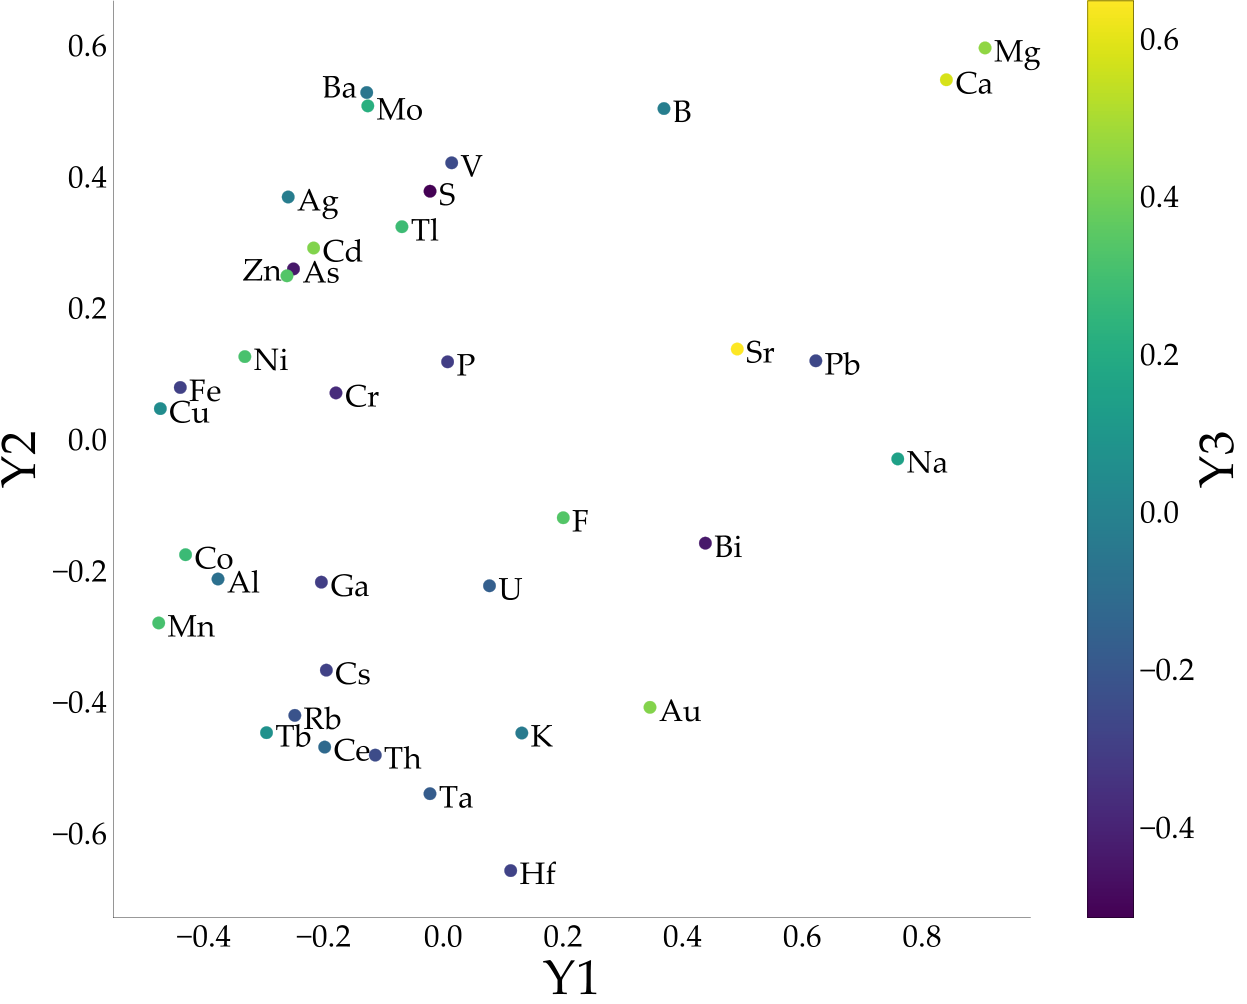
\includegraphics[scale=0.25]{gambar/MD}
          \caption{scatter plot multidimensional scaling}
          \label{md}
      \end{figure}


  \subsection{Python}
    \indent Python adalah sebuah bahasa pemrograman komputer berbasis interpreter. Python banyak dimanfaatkan diberbagai bidang. Mulai dari bidang \emph{web programming}, aplikasi desktop, \emph{backend programming} sampai dengan komputasi saintifik dan \emph{machine learning}. Python memiliki keunggulan yaitu syntax yang sederhana dan mudah dimengerti. Sehingga orang awam yang sebelumnya melakukan pemrograman komputer sangat disarankan menggunakan python untuk belajar karena mudah untuk dimengerti dan diaplikasikan.\\
    \indent keunggulan lain dari python adalah python memiliki fleksibilitas untuk menggunakan \emph{package} yang dapat memudahkan pengguna. Ini menjadi daya tarik utama untuk pengguna menggunakan python karena mereka tidak perlu menulis kode benar-benar dari nol. Mereka hanya perlu memanggil fungsi yang diinginkan dari \emph{package} yang bersangkutan.\\
    \indent Semua kemudahan yang datang bersama python tidak datang tanpa kekurangan. Python memiliki kekurangan yaitu waktu untuk mengeksekusi program yang relatif lebih lama dibandingkan bahasa pemrograman dengan basis compiler. Hal ini dikarenakan python berbasis interpreter sehingga dalam proses eksekusi program berlangsung secara baris per baris. Jadi dikembalikan lagi kepada kebutuhan dari si pengguna. Apabila pengguna membutuhkan performa yang cepat tidak disarankan menggunakan python tetapi apabila pengguna akan melakukan analisis yang kompleks sangat disarankan menggunakan python. \\
    
    \begin{figure}[H]
    	\centering
    	
\includegraphics[scale=0.5]{gambar/py}
    	\caption{logo python}
    	\label{py}
    \end{figure}

% Baris ini digunakan untuk membantu dalam melakukan sitasi
% Karena diapit dengan comment, maka baris ini akan diabaikan
% oleh compiler LaTeX.
\begin{comment}
\bibliography{daftar-pustaka}
\end{comment}


%!TEX root = ./template-skripsi.tex
%-------------------------------------------------------------------------------
%                            BAB III
%               		METODOLOGI PENELITIAN
%-------------------------------------------------------------------------------

\chapter{METODOLOGI PENELITIAN}

\section{Alat dan Bahan}
	Alat dan bahan yang digunakan pada penelitian ini terbagi atas perangkat keras dan perangkat lunak yang akan dijelaskan seperti berikut.

	\subsection{Perangkat Keras}
		Pro omnium incorrupte ea. Elitr eirmod ei qui, ex partem causae disputationi nec. Amet dicant no vis, eum modo omnes quaeque ad, antiopam evertitur reprehendunt pro ut. Nulla inermis est ne. Choro insolens mel ne, eos labitur nusquam eu, nec deserunt reformidans ut. His etiam copiosae principes te, sit brute atqui definiebas id.

		\vspace{-0.5cm}

		\begin{enumerate}[a.]
		\begin{singlespace}
		\itemsep0em
			\item Kit pancar-rima IQRF TR-53B (3 unit),
			\item Kit pengunduh program CK-USB-04 (1 unit),
			\item Kit pengembangan DK-EVAL-03 (2 unit),
			\item Kit pengembangan CK-EVAL-04 (1 unit),
			\item \emph{XBee 802.15.4 Radios (Series 1)} (3 unit),
			\item \emph{XBee Explorer USB Board} (1 unit),
			\item \emph{2 channel Relay Shield For Arduino (With XBee/BTBee interface)} (2 unit),
			\item Arduino Uno (2 unit),
			\item TP-LINK MR3020 (1 unit),
			\item Kabel USB ke Serial Prolific (1 unit).
		\end{singlespace}
		\end{enumerate}

	\subsection{Perangkat Lunak}
		Pro omnium incorrupte ea. Elitr eirmod ei qui, ex partem causae disputationi nec. Amet dicant no vis, eum modo omnes quaeque ad, antiopam evertitur reprehendunt pro ut. Nulla inermis est ne. Choro insolens mel ne, eos labitur nusquam eu, nec deserunt reformidans ut. His etiam copiosae principes te, sit brute atqui definiebas id.

		\vspace{-0.5cm}

		\begin{enumerate}[a.]
		\begin{singlespace}
		\itemsep0em
			\item Arduino for Mac OS X,
			\item CoolTerm,
			\item Driver FTDI for Mac OS X,
			\item PHP, MySQL, dan uHTTPd,
			\item Python dan pustaka PySerial,
			\item IQRF IDE v 2.08 for TR-53B,
			\item SSHFS,
			\item Sublime Text 3.
		\end{singlespace}
		\end{enumerate}

\section{Alur Penelitian}
	Consul graeco signiferumque qui id, usu eu summo dicunt voluptatum, nec ne simul perpetua posidonium. Eos ea saepe prodesset signiferumque. No dolore possit est. Mei no justo intellegebat definitiones, vis ferri lorem eripuit ad. Solum tritani scribentur duo ei, his an adipisci intellegat.

\section{Tahapan Pelaksanaan}
	Consul graeco signiferumque qui id, usu eu summo dicunt voluptatum, nec ne simul perpetua posidonium. Eos ea saepe prodesset signiferumque. No dolore possit est. Mei no justo intellegebat definitiones, vis ferri lorem eripuit ad. Solum tritani scribentur duo ei, his an adipisci intellegat.

\section{Jadwal Kegiatan}
	Quo no atqui omnesque intellegat, ne nominavi argumentum quo. Eum ei purto oporteat dissentiet, soleat utamur an sit. Et assum dicam interpretaris quo. Cetero alterum ea vel, no possit alterum utroque nec. His fuisset quaestio ad. Has eu tritani incorrupte consequuntur, esse aliquip nec ne \ref{jadwal}.

	% Please remember to add \use{multirow} to your document preamble in order to suppor multirow cells
		\begin{table}[H]
		\centering
		\caption{Jadwal Penelitian.}
		\label{jadwal}
		\begin{tabular}{|c|l|l|l|l|l|l|l|}
		\hline
		\multirow{2}{*}{No} & \multirow{2}{*}{Keterangan} & \multicolumn{6}{c|}{Bulan}                                                                                                                          \\ \cline{3-8} 
		                    &                             & 1 & 2 & 3 & 4 & 5 & 6 \\ \hline
		1                   & Studi literatur                                  &\cellcolor{gray} &\cellcolor{gray}&                        &                        &                        &                         \\ \hline
		2                   & Desain                                           &                        &\cellcolor{gray}&\cellcolor{gray}&                        &                        &                         \\ \hline
		3                   & Pembelian bahan                                  &                        &                        &\cellcolor{gray}&                        &                        &                         \\ \hline
		4                   & Pembuatan prototipe                              &                        &                        &\cellcolor{gray}&\cellcolor{gray}&\cellcolor{gray}&                         \\ \hline
		5                   & Uji coba dan perbaikan                           &                        &                        &                        &\cellcolor{gray}&\cellcolor{gray}&                         \\ \hline
		6                   & Penulisan skripsi                                &                        &                        &                        &                        &                        &\cellcolor{gray}\\ \hline
		\end{tabular}
		\end{table}
	
% Baris ini digunakan untuk membantu dalam melakukan sitasi
% Karena diapit dengan comment, maka baris ini akan diabaikan
% oleh compiler LaTeX.
\begin{comment}
\bibliography{daftar-pustaka}
\end{comment}


%!TEX root = ./template-skripsi.tex
%-------------------------------------------------------------------------------
%                            BAB IV
%               		HASIL DAN PEMBAHASAN
%-------------------------------------------------------------------------------

\chapter{HASIL DAN PEMBAHASAN}
	\section{Subbab 1}
		Habeo perfecto in sea. Ea deleniti gloriatur pri, paulo mediocrem incorrupte sea ei. Ad mollis scripta per. Incorrupte sadipscing ne mel. Mel ex nonumy malorum epicurei.

		Ne per tota mollis suscipit. Ullum labitur vim ut, ea dicit eleifend dissentias sit. Duis praesent expetenda ne sed. Sit et labitur albucius elaboraret. Ceteros efficiantur mei ad. Hendrerit vulputate democritum est at, quem veniam ne has, mea te malis ignota volumus.

		Eros reprimique vim no. Alii legendos volutpat in sed, sit enim nemore labores no. No odio decore causae has. Vim te falli libris neglegentur, eam in tempor delectus dignissim, nam hinc dictas an.
	
	\section{Subbab 2}		
		Habeo perfecto in sea. Ea deleniti gloriatur pri, paulo mediocrem incorrupte sea ei. Ad mollis scripta per. Incorrupte sadipscing ne mel. Mel ex nonumy malorum epicurei.

		\subsection{Subsubbab 2 1}
			Ne per tota mollis suscipit. Ullum labitur vim ut, ea dicit eleifend dissentias sit. Duis praesent expetenda ne sed. Sit et labitur albucius elaboraret. Ceteros efficiantur mei ad. Hendrerit vulputate democritum est at, quem veniam ne has, mea te malis ignota volumus.
			
			\begingroup
			    \fontsize{10pt}{12pt}\selectfont
			    \begin{verbatim}
					config mount
				        option target        /mnt
				        option device        /dev/sda1
				        option fstype        ext3
				        option options       rw,sync
				        option enabled       1
				        option enabled_fsck  0
				        option is_rootfs     1
			    \end{verbatim}  
			\endgroup

			\begingroup
			    \fontsize{10pt}{12pt}\selectfont
			    \begin{verbatim}
					# opkg update
					# opkg install python pyserial
			    \end{verbatim}  
			\endgroup			

		\subsection{Subsubbab 2 2}
			Consul graeco signiferumque qui id, usu eu summo dicunt voluptatum, nec ne simul perpetua posidonium. Eos ea saepe prodesset signiferumque. No dolore possit est. Mei no justo intellegebat definitiones, vis ferri lorem eripuit ad. Solum tritani scribentur duo ei, his an adipisci intellegat.

	\section{Subab 3}
		Consul graeco signiferumque qui id, usu eu summo dicunt voluptatum, nec ne simul perpetua posidonium. Eos ea saepe prodesset signiferumque. No dolore possit est. Mei no justo intellegebat definitiones, vis ferri lorem eripuit ad. Solum tritani scribentur duo ei, his an adipisci intellegat.
			
			
% Baris ini digunakan untuk membantu dalam melakukan sitasi.
% Karena diapit dengan comment, maka baris ini akan diabaikan
% oleh compiler LaTeX.
\begin{comment}
\bibliography{daftar-pustaka}
\end{comment}

%!TEX root = ./template-skripsi.tex
%-------------------------------------------------------------------------------
%                            	BAB V
%               		KESIMPULAN DAN SARAN
%-------------------------------------------------------------------------------

\chapter{KESIMPULAN DAN SARAN}

\section{Kesimpulan}
	Berdasarkan hasil analisis dan pengujian fungsional aplikasi ini, didapat kesimpulan sebagai berikut:

	\begin{enumerate}
		\item Lorem ipsum is a pseudo-Latin text used in web design, typography, layout, and printing in place of English to emphasise design elements over content. 
		
		\item It's also called placeholder (or filler) text. It's a convenient tool for mock-ups. 
		
		\item It helps to outline the visual elements of a document or presentation, eg typography, font, or layout. Lorem ipsum is mostly a part of a Latin text by the classical author and philospher Cicero.

		\item Its words and letters have been changed by addition or removal, so to deliberately render its content nonsensical; it's not genuine, correct, or comprehensible Latin anymore. 
	\end{enumerate}


\section{Saran}
	\begin{enumerate}
		\item Lorem ipsum is a pseudo-Latin text used in web design, typography, layout, and printing in place of English to emphasise design elements over content. 
		
		\item It's also called placeholder (or filler) text. It's a convenient tool for mock-ups. 
		
		\item It helps to outline the visual elements of a document or presentation, eg typography, font, or layout. Lorem ipsum is mostly a part of a Latin text by the classical author and philospher Cicero.

		\item Its words and letters have been changed by addition or removal, so to deliberately render its content nonsensical; it's not genuine, correct, or comprehensible Latin anymore. 
	\end{enumerate}

	
% Baris ini digunakan untuk membantu dalam melakukan sitasi
% Karena diapit dengan comment, maka baris ini akan diabaikan
% oleh compiler LaTeX.
\begin{comment}
\bibliography{daftar-pustaka}
\end{comment}


%-----------------------------------------------------------------
%Disini akhir masukan Bab
%-----------------------------------------------------------------


%-----------------------------------------------------------------
% Disini awal masukan untuk Daftar Pustaka
% - Daftar pustaka diambil dari file .bib yang ada pada folder ini
%   juga.
% - Untuk memudahkan dalam memanajemen dan menggenerate file .bib
%   gunakan reference manager seperti Mendeley, Zotero, EndNote,
%   dll.
%-----------------------------------------------------------------
\bibliography{library}
\addcontentsline{toc}{chapter}{DAFTAR PUSTAKA}
%-----------------------------------------------------------------
%Disini akhir masukan Daftar Pustaka
%-----------------------------------------------------------------

\end{document}